\chapter{Introdução}
\label{cap:introducao}
% --------------------------------------------------------------------------

\section{Contextualização histórica e a revolução dos pequenos satélites}
\label{sec:intro-contexto}

A democratização do acesso à órbita baixa terrestre (\textit{Low Earth Orbit} -- LEO), impulsionada pioneiramente no final da década de 1990 pelo padrão \textit{CubeSat Design Specification} (CDS) formulado pela California Polytechnic State University e pela Stanford University (CALIFORNIA POLYTECHNIC STATE UNIVERSITY, 2022), transformou profundamente a economia e a dinâmica de engenharia do setor espacial. Ao substituir plataformas satelitais monolíticas de grande porte — historicamente associadas a orçamentos de centenas de milhões de dólares e ciclos de desenvolvimento decenais — por plataformas miniaturizadas, modulares e padronizadas em unidades cúbicas fundamentais de \SI{100.0}{\milli\metre} de aresta e massa nominal unitária da ordem de \SI{1.33}{\kilo\gram} (definindo o fator de forma 1U), abriu-se caminho para constelações distribuídas, missões de sensoriamento remoto ágil e testes orbitais de cargas úteis científicas a custos e prazos ordens de magnitude inferiores.

No entanto, a miniaturização extrema e a consolidação do padrão CubeSat trouxeram contrapartidas severas no domínio da confiabilidade mecânica e da integridade física de subsistemas eletrônicos. Investigações empíricas e levantamentos estatísticos globais de missões de nanossatélites — tais como a base histórica de dados de falhas de CubeSats mantida por Swartwout (2023) e auditorias de confiabilidade conduzidas pela Agência Espacial Europeia (ESA) e pela NASA — revelam um cenário de risco expressivo: aproximadamente \SIrange{35}{45}{\percent} dos nanossatélites lançados na última década enfrentaram falha prematura nas primeiras semanas em órbita ou sequer chegaram a estabelecer contato após a ejeção do lançador (\textit{Dead on Arrival} -- DoA). 

Embora falhas de software e esgotamento precoce de baterias figurem com frequência nos diagnósticos preliminares, análises forenses aprofundadas demonstram que uma parcela substancial das anomalias tem gênese em danos estruturais silenciosos acumulados durante as etapas dinâmicas de ascensão no foguete e separação do dispensador: trincas por fadiga em juntas soldadas de componentes montados em superfície (SMD), afrouxamento ou falha de conectores interplacas (\textit{bus} PC/104), desalinhamento de sensores ópticos e solares, e travamento cinemático (\textit{jamming}) de mecanismos articulados ou de ejeção causados por deformações plásticas residuais do chassi primário (SLEJKO \textit{et al.}, 2023).

A Figura~\ref{fig:itasat} ilustra a arquitetura estrutural e a densidade interna de subsistemas do nanossatélite universitário brasileiro ITASAT-1 (CARRARA \textit{et al.}, 2017), desenvolvido conjuntamente pelo Instituto Tecnológico de Aeronáutica (ITA) e pelo Instituto Nacional de Pesquisas Espaciais (INPE). Observa-se que a estrutura primária do CubeSat atua como a espinha dorsal de suporte mecânico para placas aviônicas, baterias, sistemas de controle de atitude (rodas de reação e magnetotorquers) e experimentos de carga útil. Nesse ambiente ultracompacto, não há espaço volumétrico disponível para a instalação de subsistemas convencionais dedicados de isolamento vibratório — tais como amortecedores elastoméricos de base ou isoladores de cabo de aço (\textit{wire rope isolators}) —, os quais, ademais, sofrem degradação por perda de massa volátil em alto vácuo (\textit{outgassing}) e variação drástica de rigidez sob os ciclos térmicos orbitais severos de LEO (\SIrange{-40}{+85}{\celsius}).

\begin{figure}[htb]
  \caption{Arranjo estrutural e distribuição de subsistemas do nanossatélite universitário ITASAT-1}
  \label{fig:itasat}
  \begin{center}
    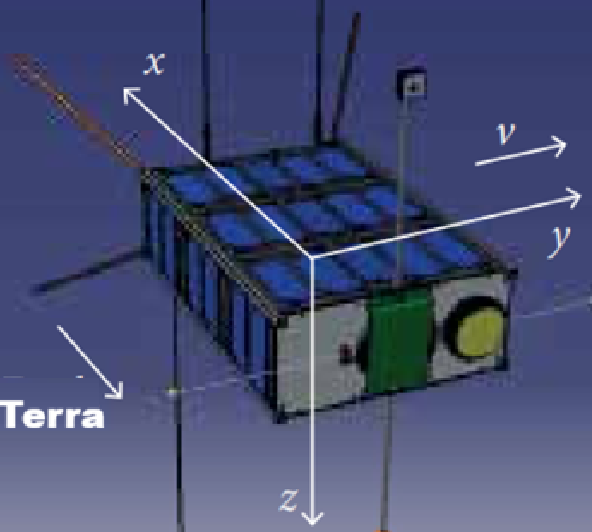
\includegraphics[width=0.75\textwidth]{figuras/itasat1_estrutura.png}
  \end{center}
  \fonte{Adaptado de Carrara \textit{et al.} (2017).}
\end{figure}

\section{O ambiente dinâmico de lançamento e as interfaces de confinamento}
\label{sec:intro-ambiente}

Durante a trajetória de ascensão do veículo lançador, a estrutura do nanossatélite é submetida a um dos ambientes mecânicos mais severos da engenharia aeroespacial. Esse regime decorre da sobreposição de três fontes primárias de excitação:
\begin{alineas}
  \item \textbf{cargas quase estáticas e de manobra:} acelerações axiais e transversais contínuas resultantes do empuxo dos motores do foguete e de manobras aerodinâmicas guiadas na atmosfera densa, impondo níveis de carga estática equivalente da ordem de \SIrange{10}{20}{\gacc};
  \item \textbf{vibrações acústicas e aerodinâmicas aleatórias:} ruído acústico gerado pela pluma dos motores químicos no momento da decolagem e ondas de pressão turbulenta geradas na camada limite durante a transição transônica e na passagem pela máxima pressão dinâmica (\textit{Max-Q}), as quais penetram a coifa protetora do foguete e excitam a base do satélite sob um espectro estocástico de banda larga (\SIrange{20}{2000}{\hertz});
  \item \textbf{choques mecânicos pirotécnicos e de separação:} pulsos transientes de curta duração gerados pela detonação de parafusos pirotécnicos nas etapas de separação de estágios e ejeção da coifa, seguidos pelo choque impulsivo gerado pela mola do dispensador orbital no instante da liberação.
\end{alineas}

Para garantir que satélites secundários não sofram colapso estrutural nem representem risco de desprendimento para a carga útil principal ou para o lançador, as agências espaciais e operadoras de lançamento impõem normas de qualificação estritas. No âmbito da NASA e de programas espaciais correlatos, a referência canônica mandatória é a norma \textit{General Environmental Verification Standard} (GEVS) (NASA, 2013), consubstanciada no documento NASA GSFC-STD-7000A. A norma estabelece que cargas úteis e subsistemas qualificados para voo devem ser testados sob um perfil de Densidade Espectral de Potência (PSD) de vibração aleatória com valor global de aceleração eficaz de
\begin{equation}
  \Grmsbase = \SI{14.1}{\Grms}
  \label{eq:intro-grms}
\end{equation}
na faixa de \SIrange{20}{2000}{\hertz}, com duração contínua de \SI{120.0}{\second} ao longo de cada um dos três eixos ortogonais ($X, Y, Z$). 

Em consonância com essas diretrizes internacionais, a Agência Espacial Brasileira (AEB, 2026), em sua \textit{Apostila da Temática -- Projeto Estrutural de Nanossatélites}, preconiza que qualquer estrutura primária destinada a voo deve possuir rigidez elástica suficiente para garantir desacoplamento dinâmico perante os modos fundamentais do foguete, estipulando que a primeira frequência natural fundamental em configuração de lançamento deve satisfazer:
\begin{equation}
  f_1 \ge \SI{100.0}{\hertz}
  \label{eq:intro-f1}
\end{equation}
Essa restrição inferior de \SI{100.0}{\hertz} impede o fenômeno de ressonância mecânica global com as oscilações de baixa frequência induzidas pela instabilidade de combustão dos motores do foguete (efeito pogo) e pelas manobras de controle de guiagem.

\section{Interface com o dispensador P-POD e restrições cinemáticas estritas}
\label{sec:intro-ppod}

Investigações dinâmicas e de integração desenvolvidas no âmbito de projetos espaciais brasileiros, como a missão SPORT (\textit{Scintillation Prediction Observations Research Task}) (SANTOS \textit{et al.}, 2020) — satélite CubeSat 6U desenvolvido conjuntamente pelo ITA, INPE, NASA Marshall Space Flight Center e The Aerospace Corporation —, destacam a centralidade da interface de acoplamento mecânico com o mecanismo de ejeção. O padrão mais difundido e maduro para lançamento de CubeSats é o dispensador \textit{Poly-Picosatellite Orbital Deployer} (P-POD), desenvolvido pela California Polytechnic State University (PUIG-SUARI; TURNER; AHLGREN, 2002), cuja interface mecânica está esquematizada na Figura~\ref{fig:interface}.

\begin{figure}[htb]
  \caption{Interface mecânica e cinemática de contato entre os trilhos do CubeSat e o dispensador orbital P-POD durante o curso de ejeção}
  \label{fig:interface}
  \begin{center}
    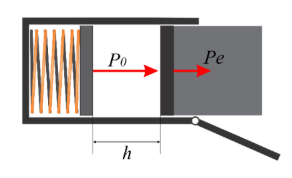
\includegraphics[width=0.65\textwidth]{figuras/interface_cubesat_deployer.png}
  \end{center}
  \fonte{Adaptado de Santos \textit{et al.} (2020).}
\end{figure}

O mecanismo cinemático do P-POD fundamenta-se no confinamento do CubeSat no interior de um tubo retangular de paredes de alumínio. O satélite apoia-se axialmente em uma placa empurradora conectada a uma mola helicoidal principal pré-carregada. No momento da ejeção orbital, as portas do dispensador abrem-se via atuador térmico ou queima de fio fusível, liberando a mola que empurra o satélite ao longo do tubo lançador. Esse mecanismo impõe exigências construtivas intransponíveis à arquitetura mecânica do satélite:
\begin{alineas}
  \item \textbf{continuidade e solidez dos trilhos-guia:} os quatro cantos longitudinais do CubeSat atuam como patins deslizantes em contato direto metal-metal contra as guias internas do dispensador. Por exigência da CDS Rev. 14 (CALIFORNIA POLYTECHNIC STATE UNIVERSITY, 2022), esses trilhos devem possuir largura mínima de \rail{}, continuidade longitudinal total ao longo dos \SI{113.5}{\milli\metre} de altura e cantos com raio de arredondamento $R \ge \SI{1.0}{\milli\metre}$;
  \item \textbf{acabamento superficial e prevenção de soldagem a frio:} para assegurar coeficiente de atrito cinemático baixo e controlado ($\mu \approx \num{0.20}$), evitar travamento mecânico por engripamento (\textit{jamming}) e prevenir a microssoldagem a frio (\textit{cold welding}) das superfícies metálicas em vácuo espacial profundo, os trilhos devem receber tratamento superficial de anodização dura Tipo III (PTFE impregnado) com rugosidade controlada $Ra \le \SI{1.6}{\micro\metre}$;
  \item \textbf{confinamento com folga lateral (\textit{clearance}):} a interface trilho-canaleta opera com folga dimensional nominal de projeto na faixa de \SIrange{0.1}{0.3}{\milli\metre}. Essa folga impede o engastamento rígido do satélite durante o lançamento, resultando em contato unilateral não linear, batimento mecânico intermitente (\textit{chattering}) e redistribuição dinâmica de esforços nos cantos do chassi.
\end{alineas}

Essa realidade cinemática dita uma decisão de engenharia mandatória: \textbf{os trilhos externos do CubeSat não podem ser aliviados, vazados ou descontinuados}. Consequentemente, qualquer esforço de redução de massa estrutural e qualquer mecanismo de isolamento e amortecimento dinâmico passivo devem ser concentrados estritamente nos painéis internos e nas paredes estruturais do chassi.

\section{Gargalos dos chassis convencionais e a promessa dos metamateriais auxéticos}
\label{sec:intro-metamateriais}

Historicamente, os chassis primários de CubeSats têm sido fabricados por usinagem subtrativa CNC a partir de blocos monolíticos maciços de ligas de alumínio convencionais, como a liga de Al 6061-T6. Embora tais ligas apresentem comportamento elastoplástico amplamente documentado e excelente usinabilidade, estruturas monolíticas usinadas sofrem de graves limitações sob dinâmica de vibração aleatória:
\begin{enumerate}
  \item \textbf{elevada massa estrutural parasitária:} a necessidade de manter espessuras mínimas de usinagem e nervuras de reforço contínuas resulta em massas de chassi da ordem de \SIrange{0.280}{0.350}{\kilo\gram}, consumindo mais de \SI{25}{\percent} do orçamento total de massa permitido para um satélite 1U (\SI{1.33}{\kilo\gram});
  \item \textbf{acoplamento dinâmico rígido direto e baixa dissipação:} corpos metálicos monolíticos possuem amortecimento histerético intrínseco extremamente baixo ($\zeta \le \SI{1.0}{\percent}$, ou seja, fator de qualidade na ressonância $Q \ge 50$). Isso significa que o chassi atua como um amplificador mecânico rígido, transferindo praticamente sem atenuação a densidade espectral de potência (PSD) da base diretamente para as placas eletrônicas e cargas úteis sensíveis instaladas em seu interior (SLEJKO \textit{et al.}, 2023).
\end{enumerate}

Como alternativa transformadora a essa limitação física, a pesquisa contemporânea na fronteira da ciência dos materiais e mecânica dos sólidos tem convergido para o uso de \textbf{metamateriais celulares arquitetados com coeficiente de Poisson negativo ($\nu < 0$)}, conhecidos como materiais auxéticos (LI \textit{et al.}, 2026). Diferentemente de materiais convencionais — que sofrem afilamento transversal quando tracionados longitudinalmente —, as estruturas celulares auxéticas exibem expansão lateral quando tracionadas e contração lateral quando comprimidas, fenômeno governado pela cinemática interna de rotação e flexão de costelas celulares reentrantes.

Essa cinemática celular singular confere aos metamateriais auxéticos um conjunto de propriedades mecânicas excepcionais para aplicações aeroespaciais (FARSHBAF \textit{et al.}, 2025; CUI \textit{et al.}, 2025):
\begin{alineas}
  \item \textbf{elevada Absorção Específica de Energia (\textit{Specific Energy Absorption} -- SEA):} capacidade de dissipar grandes quantidades de energia mecânica deformacional por unidade de massa em virtude do colapso volumétrico confinado e da redistribuição de momentos fletores nas hastes oblíquas;
  \item \textbf{resistência superior à indentação e tenacidade à fratura:} o fechamento lateral das células em torno de pontos de aplicação concentrada de carga promove redistribuição estática de tensões;
  \item \textbf{atenuação vibroacústica no regime sub-comprimento de onda:} a microarquitetura celular confere mecanismos extraordinários de atenuação dinâmica passiva decorrentes do severo descasamento de impedância acústica entre os trilhos sólidos ($Z_{\text{solid}} \approx \SI{13.47}{\mega\pascal\second\per\metre}$) e o núcleo celular ($Z_{\text{eff}} \approx \SI{1.39}{\mega\pascal\second\per\metre}$), associado a antirressonâncias mecânicas locais induzidas pela flexão distribuída das costelas e ao desacoplamento cinemático de modos de tombamento (\textit{rocking}) proporcionado pelo coeficiente de Poisson negativo;
\end{alineas}

\section{Manufatura Aditiva Metálica (L-PBF) e as barreiras computacionais de dimensionamento}
\label{sec:intro-dfam-ia}

A viabilização física de geometrias celulares tridimensionais complexas tornou-se viável industrialmente devido ao amadurecimento dos processos de Manufatura Aditiva por Fusão em Leito de Pó a Laser (\textit{Laser Powder Bed Fusion} -- L-PBF), também conhecida como \textit{Selective Laser Melting} (SLM), na liga aeroespacial AlSi10Mg. No entanto, a síntese de componentes celulares via L-PBF exige a obediência irrestrita aos princípios de Projeto para Manufatura Aditiva (\textit{Design for Additive Manufacturing} -- DfAM) (KHAN; RICCIO, 2024):
\begin{alineas}
  \item \textbf{auto-suporte de superfícies suspensas:} superfícies inclinadas em relação à mesa de construção devem manter ângulo $\theta_{\text{overhang}} \ge \SI{35}{\degree}$ para prevenir colapso da poça de fusão por gravidade e dispensar suportes internos sacrificiais inacessíveis;
  \item \textbf{espessura mínima de costela e efeito de casca (\textit{skin effect}):} a espessura de parede deve obedecer ao limite tecnológico $t \ge \SI{0.60}{\milli\metre}$ para evitar defeitos de falta de fusão (\textit{lack of fusion}). Adicionalmente, a rugosidade superficial típica $Ra \in [10, 18]\ \mu\text{m}$ (atingindo $Ra \approx \SI{25}{\micro\metre}$ em faces \textit{down-skin}) reduz a seção portante efetiva em $\sim 8 - 10\%$, exigindo pós-processamento por usinagem por fluxo abrasivo (AFM) ou eletropolimento ($Ra < \SI{3.2}{\micro\metre}$) para o hardware de voo;
  \item \textbf{desobstrução de canais de evacuação de pó:} todos os vazios internos devem possuir canais de alívio contínuos com orifícios de purga $d_{\text{drain}} \ge \SI{2.0}{\milli\metre}$ para a extração do pó metálico não consolidado após a queima a laser.
\end{alineas}

Entretanto, o dimensionamento ótimo e a exploração do vasto espaço de projeto dessas estruturas celulares esbarram em um obstáculo de custo computacional intransponível: a análise elastodinâmica tridimensional de uma única geometria celular por Elementos Finitos (FEA) de alta fidelidade — discretizada com centenas de milhares de elementos tetraédricos de segunda ordem (Tet10) para resolver as costelas delgadas e junções nodais — demanda tempos de processamento da ordem de minutos a horas em clusters de computação de alto desempenho (HPC). Em contrapartida, algoritmos de otimização evolutiva multiobjetivo (como o NSGA-II) exigem dezenas de milhares de avaliações funcionais para convergir à fronteira de Pareto ótima, tornando o acoplamento direto entre FEA 3D e otimização totalmente impraticável (tempo estimado em semanas ou meses de processamento ininterrupto).

Para transpor essa barreira sem recorrer a simplificações grosseiras de caixa preta, esta pesquisa concebe uma esteira computacional inovadora que combina:
\begin{enumerate}
  \item Modelagem analítica multiescala e leis de escala corrigidas de Gibson-Ashby (1997) e Beigrezaee \textit{et al.} (2026);
  \item Treinamento de um Modelo Substituto Neural Profundo com Conexões Residuais Guiado por Leis Físicas (\textit{Physics-Guided ResNet}), cuja função de perda composta incorpora penalidades fenomenológicas que impedem extrapolações espúrias e garantem monotonicidade elástica estrita;
  \item Orquestração por Grafo de Estados Finitos Determinístico (LangGraph) sob tipagem forte em Python puro, com descarte antecipado (\textit{fail-fast}) de geometrias que violem as restrições de DfAM;
  \item Otimização multiobjetivo via algoritmo genético NSGA-II acoplado ao método de tomada de decisão multicritério TOPSIS para identificação da geometria de compromisso ótimo;
  \item Validação de alta fidelidade (\textit{Ground Truth}) com o solver aberto Code\_Aster (EDF), verificação cruzada com o CalculiX, e dinâmica explícita não linear com o OpenRadioss para qualificação ao choque de ejeção no dispensador P-POD.
\end{enumerate}

\section{Problema de pesquisa, hipóteses científicas e critérios de sucesso}
\label{sec:intro-problema}

Diante das limitações do estado da arte e das severas exigências espaciais, o problema fundamental de engenharia que norteia esta investigação é formulado nos seguintes termos:
\begin{quote}
  \textit{Como conceber, otimizar e qualificar a arquitetura estrutural primária de um nanossatélite CubeSat 1U em liga metálica aeroespacial AlSi10Mg fabricado por Manufatura Aditiva L-PBF, integrando painéis celulares auxéticos reentrantes a trilhos monolíticos de contato, de modo a maximizar o isolamento elastodinâmico passivo das vibrações aleatórias de lançamento sobre a carga útil e minimizar a massa estrutural, sem violar as restrições normativas de rigidez fundamental ($f_1 \ge \SI{100.0}{\hertz}$), de envelope dimensional e de vida em fadiga sob o perfil estocástico da norma NASA GSFC-STD-7000A?}
\end{quote}

Para responder a essa questão, formulam-se três hipóteses científicas de trabalho, as quais serão submetidas a teste rigoroso e verificação quantitativa ao longo da monografia:
\begin{alineas}
  \item \textbf{Hipótese 1 (Isolamento dinâmico passivo no regime sub-comprimento de onda):} A incorporação de painéis celulares auxéticos reentrantes tridimensionais dotados de coeficiente de Poisson efetivo negativo ($\nu_{\text{eff}} < 0$) promove forte descasamento de impedância acústica e antirressonâncias locais no regime sub-comprimento de onda ($a/\lambda \le 0{,}006 \ll 1$), resultando em uma atenuação dinâmica superior a \SI{10}{\decibel} (redução de pelo menos \SI{68}{\percent} na aceleração eficaz RMS) nas interfaces da carga útil em relação ao chassi monolítico maciço convencional, mantendo a primeira frequência natural fundamental estritamente acima do limite normativo ($f_1 \ge \SI{100.0}{\hertz}$).
  \item \textbf{Hipótese 2 (Alívio expressivo de massa com integridade mecânica de voo):} A arquitetura estrutural híbrida — combinando quatro trilhos longitudinais maciços de \rail{} (em estrito atendimento às diretrizes cinemáticas da interface P-POD) com quatro painéis laterais celulares auxéticos autossuportados ($\theta_{\text{overhang}} \ge \SI{35}{\degree}$) — viabiliza uma redução de massa de pelo menos \SI{50}{\percent} frente ao chassi usinado maciço de referência (massa estrutural $\le \SI{0.150}{\kilo\gram}$ contra $\SI{0.308}{\kilo\gram}$), assegurando Margem de Segurança estática positiva contra o escoamento ($MS_{\text{yield}} > 0$) sob o pico estocástico a $3\sigma$ e índice de dano cumulativo por fadiga de Steinberg em conformidade com o teto espacial ($D \le \num{0.25}$ sob excitação de \SI{14.1}{\Grms} durante \SI{120.0}{\second}, avaliado conservadoramente no entalhe crítico).
  \item \textbf{Hipótese 3 (Aceleração evolutiva dual por modelo substituto guiado por física):} O emprego de uma rede neural profunda com blocos residuais informada por leis fenomenológicas de Gibson-Ashby e penalidades de monotonicidade de rigidez (\textit{Physics-Guided ResNet}) viabiliza a execução de campanhas de otimização evolutiva multiobjetivo (NSGA-II) com aceleração instantânea de inferência superior a $10^5\times$ e aceleração amortizada de ponta a ponta de aproximadamente $40\times$ em comparação com a esteira direta de elementos finitos 3D, atingindo erros relativos médios inferiores a \SI{2}{\percent} na predição de frequências modais e tensões estocásticas na vizinhança da fronteira de Pareto.
\end{alineas}

\section{Delimitação de escopo e rigor metodológico}
\label{sec:intro-delimitacao}

Para assegurar honestidade intelectual e rigor científico absoluto de nível de pós-graduação, estabelecem-se com clareza as fronteiras do presente trabalho:
\begin{enumerate}
  \item \textbf{Natureza estritamente computacional e de síntese numérica:} A presente pesquisa consiste em uma investigação analítica e computacional profunda. Todas as propriedades mecânicas, tensões nodais, autovalores e transmissibilidades reportados derivam de formulações constitutivas rigorosas, mecânica do contínuo, métodos de homogeneização e simulações elastodinâmicas de elementos finitos de alta fidelidade em ambiente aberto (Code\_Aster, CalculiX, OpenRadioss e Gmsh Tet10 em Linux/WSL).
  \item \textbf{Papel circunscrito do modelo físico preliminar:} A fabricação física prévia de modelos impressos por extrusão de filamento termoplástico (PLA) circunscreveu-se unicamente a ensaios conceituais tridimensionais de empacotamento volumétrico, verificação cinemática de mecanismos de abertura de antenas e checagem dimensional de montagem (\textit{fit-check} virtual) nos trilhos do casulo lançador P-POD. Não houve realização de ensaios mecânicos de bancada (como tração uniaxial ASTM D638 ou ensaios dinâmicos em mesa vibratória). Rejeita-se categoricamente qualquer extrapolação empírica direta de propriedades dinâmicas entre polímeros e ligas metálicas, em razão da similaridade incompleta entre os materiais (módulos elásticos divergindo por mais de 25 vezes e taxas de amortecimento interno substancialmente distintas).
  \item \textbf{Ancoragem integral na liga metálica de voo e calibração de TRL:} Todo o desenvolvimento teórico, o planejamento experimental (DoE proxy calibrado), o treinamento do modelo substituto neural e os critérios de aceitação espacial (NASA GEVS) estão diretamente ancorados nas propriedades canônicas da liga aeroespacial AlSi10Mg aliviada termicamente ($300^\circ\text{C} / 2\text{ h}$), estabelecendo uma base de alta maturidade metodológica de \textbf{TRL 4 Digital (NASA SP-6105 / ESA)} para a esteira computacional e \textbf{TRL 3 Avançado de Hardware (ISO 16290:2013)}, pronta para orientar a fabricação aditiva de provetes físicos em mesa vibratória (\textbf{TRL 5}) e teste integrado em P-POD TVAC (\textbf{TRL 6}).
  \item \textbf{Foco na dinâmica estrutural e fadiga de lançamento:} O trabalho foca estritamente nas fases dinâmicas críticas de lançamento propulsivo e ejeção orbital sob temperatura ambiente de qualificação (\SI{23}{\celsius} $\pm$ \SI{3}{\celsius}). Efeitos de ciclagem térmica e termovácuo orbital profundo (TVAC, \SIrange{-40}{+85}{\celsius}), radiação ionizante e ataque por oxigênio atômico não compõem o escopo primário da presente modelagem elástica linear, sendo recomendados como diretrizes para extensões futuras.
\end{enumerate}

\section{Estrutura e organização da monografia}
\label{sec:intro-organizacao}

Para conferir clareza e encadeamento lógico à exposição da tese, o documento está estruturado em seis capítulos textuais e três apêndices técnicos:
\begin{alineas}
  \item o \textbf{Capítulo~\ref{cap:introducao} (Introdução)} contextualiza o problema, aborda as estatísticas de falha de pequenos satélites, discute o confinamento no P-POD, estabelece as hipóteses científicas e delimita o escopo da investigação;
  \item o \textbf{Capítulo~\ref{cap:objetivos} (Objetivos)} detalha formalmente o objetivo geral e desdobra as quatro fases operacionais com seus nove objetivos específicos mensuráveis;
  \item o \textbf{Capítulo~\ref{cap:revisao} (Revisão de Literatura e Fundamentos da Stack Tecnológica)} apresenta a fundamentação teórica em nanossatélites, dinâmica de lançamento, metamateriais auxéticos, DfAM, homogeneização, teoria de Bloch-Floquet, LEFM e explica exaustivamente os fundamentos operacionais de cada biblioteca e solver da esteira computacional (OpenCASCADE/build123d, Gmsh Tet10, Code\_Aster, CalculiX, OpenRadioss, LangGraph, Physics-Guided ResNet, NSGA-II e TOPSIS);
  \item o \textbf{Capítulo~\ref{cap:metodologia} (Metodologia e Procedimentos Computacionais)} detalha a formulação dimensional, as equações geométricas e de manufaturabilidade da célula, a esteira de malha Tet10 adaptativa, a arquitetura completa da rede neural guiada por física, o grafo de estados finitos e a anatomia dos decks dos solucionadores abertos;
  \item o \textbf{Capítulo~\ref{cap:resultados} (Resultados e Discussão)} expõe o estudo de convergência de malha GCI, a amostragem DoE, o treinamento da ResNet, a fronteira de Pareto NSGA-II, a decisão multicritério TOPSIS para escolha do Projeto \#28, a validação cruzada independente Code\_Aster vs CalculiX, a resposta sob vibração aleatória GEVS, a análise de integridade e fadiga estocástica de Steinberg e a qualificação ao choque no P-POD via OpenRadioss;
  \item o \textbf{Capítulo~\ref{cap:conclusao} (Conclusão e Trabalhos Futuros)} consolida as conclusões finais à luz das três hipóteses propostas, aponta os limites de validade da pesquisa e traça um roteiro tecnológico detalhado para a fabricação aditiva física e ensaios em mesa vibratória eletrodinâmica;
  \item os \textbf{Apêndices A, B e C} fornecem, respectivamente, a listagem integral dos decks de simulação dos solvers abertos, a implementação computacional do modelo substituto e do grafo LangGraph, e a tabela completa de dados do screening paramétrico e soluções de Pareto.
\end{alineas}
